Certainly! Below is a TikZ LaTeX code that generates an illustration of the type-1 triangle \( t_y \) with one of its out-edge \( e = yz \), and includes the dotted directed edges representing the edges of the cycle \( C \).

```latex
\documentclass{standalone}
\usepackage{tikz}

\begin{document}

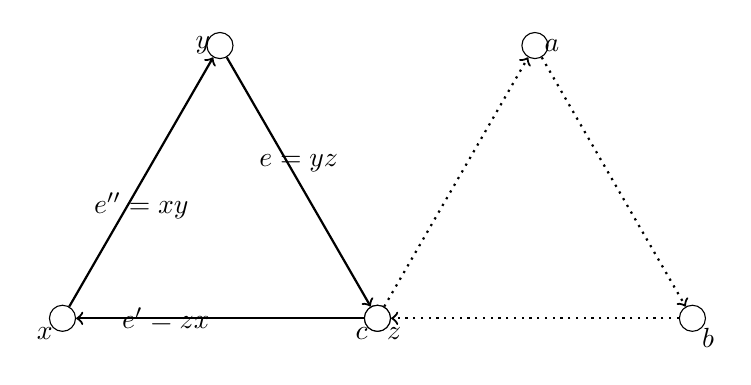
\begin{tikzpicture}[scale=2]

    % Define nodes for the triangle
    \node (y) at (0,0) [circle, draw, fill=white] {};
    \node (x) at (-1,-1.732) [circle, draw, fill=white] {};
    \node (z) at (1,-1.732) [circle, draw, fill=white] {};

    % Draw edges of the triangle
    \draw[thick, ->] (y) -- node[above] {$e=yz$} (z);
    \draw[thick, ->] (z) -- node[left] {$e' = zx$} (x);
    \draw[thick, ->] (x) -- node[below] {$e'' = xy$} (y);

    % Label vertices
    \node at (y) [left] {$y$};
    \node at (x) [below left] {$x$};
    \node at (z) [below right] {$z$};

    % Define nodes for the cycle C
    \node (a) at (2,0) [circle, draw, fill=white] {};
    \node (b) at (3,-1.732) [circle, draw, fill=white] {};
    \node (c) at (1,-1.732) [circle, draw, fill=white] {};

    % Draw edges of the cycle C
    \draw[dotted, thick, ->] (a) -- (b);
    \draw[dotted, thick, ->] (b) -- (c);
    \draw[dotted, thick, ->] (c) -- (a);

    % Label vertices of the cycle C
    \node at (a) [right] {$a$};
    \node at (b) [below right] {$b$};
    \node at (c) [below left] {$c$};

\end{tikzpicture}

\end